
\section*{Welcome reception}
We are excited to start the PuG with you on Wednesday, 7th of June, at our welcoming evening! From 6 pm on, you can get your conference documents and register onsite at the front desk at the foyer of the Tagungszentrum Morgenstelle. The evening offers an opportunity for first encounters and to meet your fellow science colleagues. Live music provides a nice ambiance to enjoy free beer, soft drinks and vegetarian/vegan food.

\section*{Social evening}
We look forward to welcoming you to the social evening on Friday at Brauwerk Freistil! The Brauwerk is known for its home-brewed beers, which, unlike its industrial counterparts, make intense flavor experiences instead of simple thirst quenching a priority.

The entrance to the social evening begins directly after the conference program at 6:30 pm. International and local finger food (including vegan options), four free drinks and the beer garden directly at the Neckar are included in the ticket price of 80€. In addition, punting boats, an ice cream and a crepe truck will be provided for a summery ambience in the beer garden. Inside Freistil, you'll find a pool table, dart and shuffle boards, as well as a foosball table to compete against your colleagues. 

From 9:15 pm on there will be live performances by the PuG band and the latin american local band Combo Cumbiale. \textbf{In a short break at around 10 pm, we will award the Poster prizes, the IGOR prize and the prize for the best supervision.} The evening is rounded up by a live set of our DJ. 

Students and PhD students can purchase a party ticket for 35€ for the later part of the evening (entrance from 9:30 pm). Two free drinks are included in the ticket price.

\begin{center}
	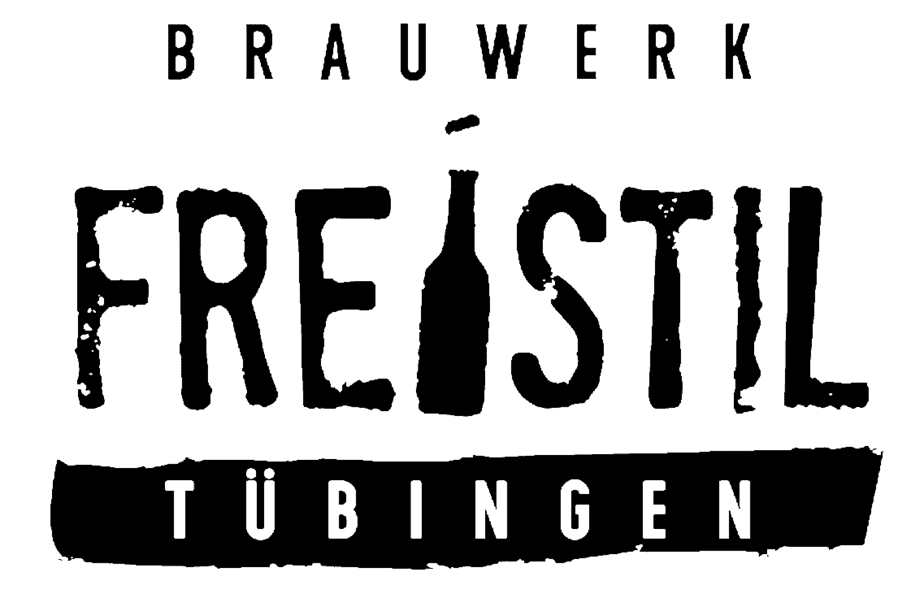
\includegraphics[width=0.3\textwidth]{tex/images/brauwerk.png}
\end{center}

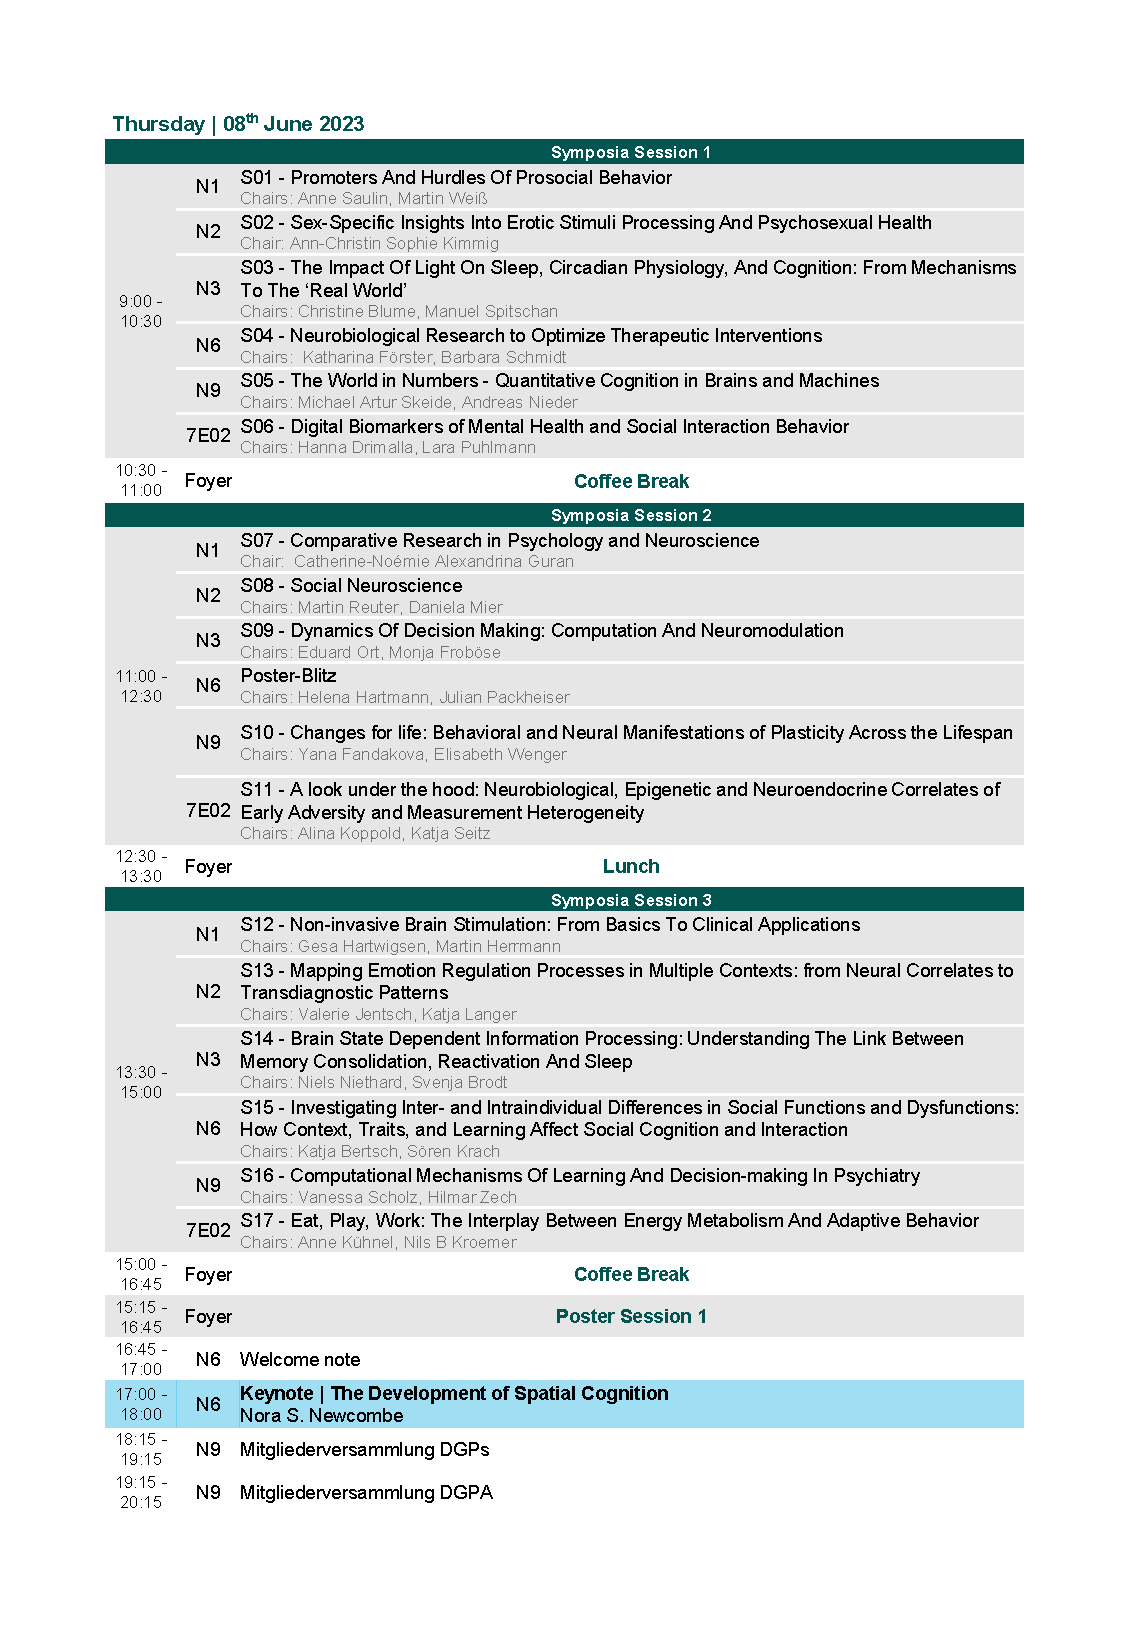
\includepdf[pages=-]{pdf_static/Program.pdf}
\includepdf[scale=0.8]{pdf_static/Social_Event_PuG}